\documentclass[10pt,a4paper]{article}
\usepackage[utf8]{inputenc}
\usepackage[spanish]{babel}
\usepackage{amsmath}
\usepackage{amsfonts}
\usepackage{amssymb}
\usepackage{makeidx}
\usepackage{graphicx}
\usepackage{lmodern}
\usepackage{kpfonts}
\usepackage{fourier}
\usepackage[hidelinks]{hyperref}
\usepackage[left=2cm,right=2cm,top=2cm,bottom=2cm]{geometry}
\author{Luis Angel Torres Pinto.\\Universidad Politécnica de la Zona Metropolitana de Guadalajara\\Ingeniería Mecatrónica. }
\title{Explicar los arreglos y parámetros de los Amplificadores Clase A}
\begin{document}
\maketitle
\centering

\includegraphics[scale=1.90]{upzmg.jpg}\\
\raggedright
\newpage
\section{Amplificadores clase A}
\part{Caracteristicas y Funcionamiento }
Un amplificador de potencia funciona en clase A cuando la tensión de polarización y la amplitud máxima de la señal de entrada poseen valores tales que hacen que la corriente de salida circule durante todo el período de la señal de entrada.\\
\centering
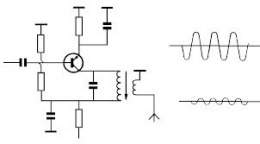
\includegraphics[scale=1]{ampli.jpg}\\
\raggedright
Son aquellos amplificador cuyas etapas de potencia consumen corrientes altas y continuas de su fuente de alimentación, independientemente de si existe señal de audio o no. Esta amplificación presenta el inconveniente de generar una fuerte y constante emisión de calor. No obstante, los transistores de salida están siempre a una temperatura fija y sin alteraciones. En general, podemos afirmar que esta clase de amplificación es frecuente en circuitos de audio y en los equipos domésticos de gama alta, ya que proporcionan una calidad de sonido potente y de muy buena calidad. Un amplificador de  clase A es aquel que presenta a su salida una señal copiada de la entrada, pero amplificada y sin distorsión. En este caso la máxima señal de salida se obtendrá cuando el punto estático coincida con el centro de la recta de carga, consiguiendo, por tanto, la máxima potencia de salida.\\
\centering
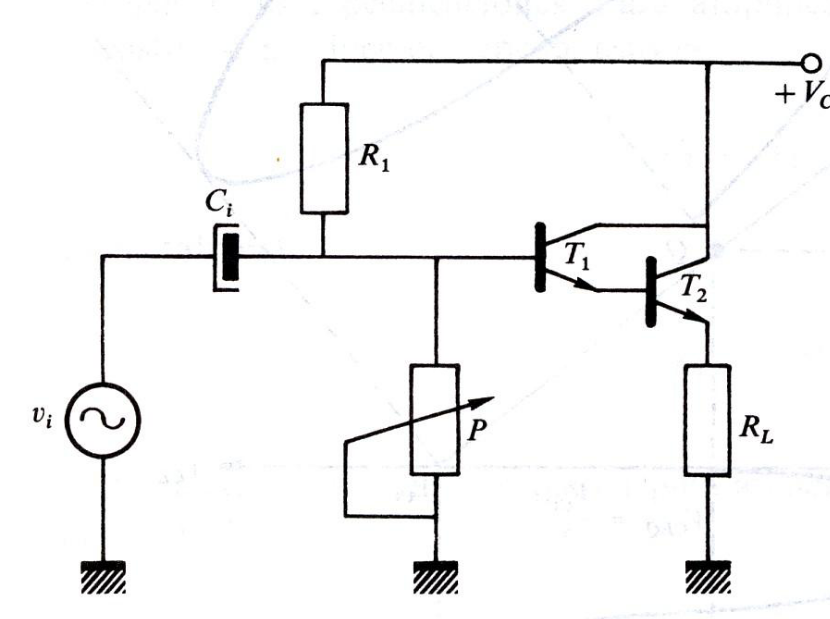
\includegraphics[scale=.40]{cir.png}  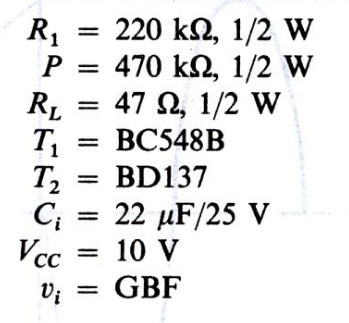
\includegraphics[scale=.30]{circu.png}\\ 
Es un par Darlington para aprovechar su elevada ganancia de corriente. En todo caso, la ganancia total obtenida será de corriente, manteniéndose la tensión de salida prácticamente al mismo nivel que la de entrada y cumpliendo, por tanto, las características de los amplificadores de  potencia.
La máxima ganancia se obtendrá cuando el Q se situe en el centro de la recta de carga. Esta será la potencia media absorbida en todo momento por el circuito de la f.a, ya que un desplazamiento del punto Q, provocado por una señal senoidal, da un valor medio <<0>> de variación de Ic.
Por otra parte, la máxima potencia disiada en la carga corresponderá al caso en que la señal de entrada provoque que el punto de trabajo recorra toda la recta de carga, esto es Vimax, dando como resultado una señal de salida de valor pico a pico, igual a Vcc y entonces dicha potencia será:\\ 
\centering
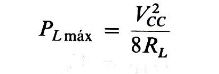
\includegraphics[scale=.50]{pote.png}\\ 
\raggedright
ya que Vcc = Vppmax, todo esto da como resultado un rendimiento\\ 
\centering
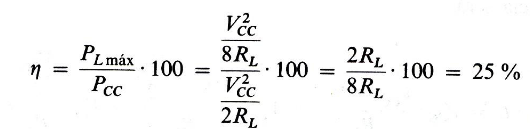
\includegraphics[scale=.50]{rend.png}\\\\
\raggedright
Se ha de tener en cuenta, que este rendimiento es el máxima que puede obtenerse en un amplificador clase A, ya que, si la señal de entrada disminuye, lo hace la tensión de salida y, por tanto, el rendimiento. Por otra parte, si la carga se acopla externamente al circuito, es decir, no es la resistencia de carga del transistor, la potencia efectiva aplicada a la carga será sólo una parte de la entregada por el circuito, disipando una parte importante la propia resistencia de carga del circuito.
Es conveniente,además, conocer la potencia que ha de disipar el transistor para no sobrepasar sus especificaciones. Para amplificadores clase A, la máxima disipación del transistor se produce en reposo, esto es,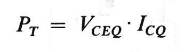
\includegraphics[scale=.80]{pt.png}\\ 
\raggedright
y, generalmente
\centering
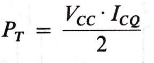
\includegraphics[scale=1]{gr.png}\\
A medida que la tensión pico a pico aumento en la carga, la potencia disipada en el transistor decrece.\\
\raggedright
\section{Ventajas}
La gran ventaja de la clase A es que es casi lineal, y en consecuencia la distorsión es menor. La gran desventaja de la clase A es que es poco eficiente, es decir que requiere un amplificador de clase A muy grande para dar 50 W, y ese amplificador usa mucha corriente y se pone a muy alta temperatura

\section{Desventajas}
La gran desventaja de la clase A es que es poco eficiente, se requiere un amplificador de clase A muy grande para dar 50 W, y ese amplificador usa mucha corriente y se pone a muy alta temperatura.
\section{Conclusión}
Resumiendo, los amplificador de clase A tienen mayor calidad de sonido, cuestan más y son menos prácticos, ya que despilfarran corriente y devuelven señales muy limpias. La clase A se refiere a una etapa de salida con una corriente de polarización mayor que la máxima corriente de salida que dan, de tal forma que los transistores de salida siempre están consumiendo corriente.La señal del transistor de salida modula tanto el voltaje como la corriente de salida. Cuando no hay señal de entrada, la corriente de polarización constante fluye directamente del positivo de la fuente de alimentación al negativo, resultando que no hay corriente de salida, se gasta mucha corriente.\\ 
\section{Referencias}
\url{https://www.forosdeelectronica.com/threads/amplificador-de-clase-a-con-2n3055.14545/}
\url{https://www.ecured.cu/Amplificador_clase_A}
\url{http://quidel.inele.ufro.cl/~jhuircan/PDF_CTOI/AmpPot20.pdf}
\end{document}